%=======================================================================
%  CSE558 Data Science - Midterm Project Report
%  Monsoon 2026, IIIT-Delhi
%=======================================================================
\documentclass[10pt,a4paper,twocolumn]{article}

\newcommand{\projecttitle}{Acoustic Dispersion and Feature Relationships\\across 17 Metal Subgenres}
\newif\ifshowhints
\showhintsfalse

%-------------------------------------------- fonts
\usepackage{iftex}
\ifPDFTeX
  \usepackage[T1]{fontenc}
  \usepackage[utf8]{inputenc}
  \IfFileExists{carlito.sty}%
    {\usepackage[sfdefault]{carlito}}%
    {\usepackage[scaled=0.92]{helvet}\renewcommand{\familydefault}{\sfdefault}}%
  \usepackage{courier}
\else
  \usepackage[no-math]{fontspec}
  \defaultfontfeatures{Ligatures=TeX}
  \IfFontExistsTF{Carlito}%
    {\setmainfont{Carlito}}%
    {\setmainfont{Helvetica}}
\fi

%----------------------------------------------------------- packages
\usepackage[margin=18mm,bottom=20mm,columnsep=7mm]{geometry}
\usepackage{amsmath,amssymb}
\usepackage{xcolor}
\usepackage{graphicx}
\usepackage{tabularx}
\usepackage{array}
\usepackage{booktabs}
\usepackage{enumitem}
\usepackage{titlesec}
\usepackage{needspace}
\usepackage[font=small,labelfont=bf]{caption}
\usepackage[hidelinks]{hyperref}
\hypersetup{pdftitle={Acoustic Dispersion and Feature Relationships across 17 Metal Subgenres},
            pdfsubject={CSE558 Data Science, Monsoon 2026: Midterm Project Report}}

%------------------------------------------------------------- layout
\definecolor{eg}{HTML}{7396C4}
\definecolor{hintgrey}{gray}{0.58}

\titleformat{\section}{\normalfont\large\bfseries}{\thesection.}{0.5em}{}
\titlespacing*{\section}{0pt}{11pt}{3pt}
\titleformat{\subsection}{\normalfont\normalsize\bfseries}{\thesubsection}{0.5em}{}
\titlespacing*{\subsection}{0pt}{9pt}{2pt}
\newcommand{\sectionbreak}{\needspace{10\baselineskip}}
\newcommand{\subsectionbreak}{\needspace{10\baselineskip}}

\setlength{\parindent}{0pt}
\setlength{\parskip}{3.5pt}
\setlist{leftmargin=1.2em, itemsep=1.5pt, topsep=1.5pt, parsep=0pt}
\renewcommand{\arraystretch}{1.2}
\setlength{\tabcolsep}{3.5pt}
\newcolumntype{L}[1]{>{\raggedright\arraybackslash}p{#1}}
\newcolumntype{Y}{>{\raggedright\arraybackslash}X}
\newcolumntype{K}[1]{>{\raggedright\arraybackslash\bfseries\boldmath}p{#1}}

%--------------------------------------------------------- shorthands
\newcommand{\code}[1]{\texttt{\small #1}}
\newcommand{\field}[2]{\textbf{#1}~#2\par}
\newcommand{\tpart}[2]{\par\needspace{9\baselineskip}\smallskip\textbf{#1)~#2}\par}
\newcommand{\minihead}[1]{\par\needspace{6\baselineskip}\smallskip\textbf{#1}\par}
\newcommand{\figfile}[2]{%
  \IfFileExists{#1}%
    {\includegraphics[width=\linewidth,height=#2,keepaspectratio]{#1}}%
    {\fbox{\parbox[c][#2][c]{\dimexpr\linewidth-2\fboxsep-2\fboxrule\relax}%
      {\centering\small\itshape\color{hintgrey}Plot: \detokenize{#1}}}}}

%=======================================================================
\begin{document}

\twocolumn[%
{\small\bfseries CSE558 Data Science\ \ \textbullet\ \ Midterm Project Report\ \ \textbullet\ \ Monsoon 2026\par}
\vspace{4pt}
{\LARGE\bfseries\raggedright\projecttitle\par}
\vspace{6pt}
\rule{\linewidth}{1pt}

{\small
\begin{tabularx}{\linewidth}{@{}K{2.4cm} Y@{}}
\toprule
Group name & 4 \\
Dataset & AcousticBrainz MediaEval features and Last.fm labels; Zenodo record 2553414 \\
Code & \url{https://github.com/Swarnav-Chakma/Metal-music-statistical-analysis} \\
\bottomrule
\end{tabularx}}

\vspace{2pt}
{\small
\begin{tabularx}{\linewidth}{@{}L{0.5cm} L{3.2cm} L{2.2cm} L{4.6cm} Y@{}}
\toprule
\textbf{\#} & \textbf{Name} & \textbf{Roll no.} & \textbf{Institute email} & \textbf{Contribution} \\
\midrule
1 & Swarnav Chakma & 2023541 & swarnav23541@iiitd.ac.in & Code repository \& implementation, statistical modelling, problem statements, Tests 1 and 2 (4, 5). \\
2 & Manas Singh & 2024330 & manas24330@iiitd.ac.in & Data preparation, code implementation \& review, version offset regression, and before-and-after tables (2, 3). \\
3 & Arshpreet Singh Gill & 2023135 & arshpreet23135@iiitd.ac.in & code implementation \& review, Test 3 (exploratory), limitations, and report proofreading (5, 6). \\
4 & Manjot Singh Saini & 2023309 & manjot23309@iiitd.ac.in & Dataset curation, code implementation \& review, shard manifest verification, and size check (1). \\
5 & Nakul Grover & 2023336 & nakul23336@iiitd.ac.in & Exploratory data analysis, code implementation \& review, and feature distribution plots (4). \\
\bottomrule
\end{tabularx}}
\vspace{10pt}
]


\section{Dataset}
\field{Source and scope:}{The local download manifest identifies \href{https://zenodo.org/records/2553414}{Zenodo record 2553414}. We analyze an extracted shard subset of AcousticBrainz MediaEval features with Last.fm crowd-tag labels, not the entire benchmark. One row represents one recording. The local cohort contains 30,388 candidate IDs; the two processed feature shards supplied 5,874 recordings across 17 metal subgenres.}
The shard metadata names training archive \texttt{train-89} and validation archive \texttt{validation-01234567} (both under the \texttt{acousticbrainz-mediaeval-features} prefix). They report 3,108 and 2,766 retained JSON records, with no missing requested IDs. The archive identifiers and recording counts are documented in the download manifest and shard logs.

\begin{tabularx}{\linewidth}{@{}Y r r@{}}\toprule
Matrix & Rows & Features\\\midrule
Raw extracted & 5,874 & 2,675\\
Retained base & 5,858 & 2,262\\
H1 acoustic representation & 5,858 & 2,234\\\bottomrule
\end{tabularx}
\field{Size requirement:}{Raw: $5{,}874\times2{,}675=15{,}712{,}950$. Retained base: $5{,}858\times2{,}262=13{,}250{,}796$. H1: $5{,}858\times2{,}234=13{,}086{,}772$. Each exceeds 3 million instance--attributes.}
These are extracted acoustic descriptors, including scalar summaries and expanded vectors/matrices. The 28 nominal key/mode columns remain available in the base matrix but are excluded from H1 distances.

\minihead{Key features and their meaning}
{\small\begin{tabularx}{\linewidth}{@{}L{2.25cm} L{1.65cm} Y@{}}\toprule
Feature & Type & Interpretation\\\midrule
Tempo (BPM) & Continuous & Estimated beat rate; H2 predictor.\\
Spectral centroid, mean & Continuous & Frequency-weighted spectral center (Hz); brightness proxy and H2 outcome.\\
Estimated minor mode & Binary & Essentia minor-mode flag; H3 outcome, not a verified musical annotation.\\
Subgenre & Nominal & One of 17 crowd-tag labels.\\
Artist / album IDs & Nominal & Dependence links, excluded from acoustic predictors.\\
MFCC/GFCC summaries & Continuous & Spectral-envelope descriptors contributing to H1.\\\bottomrule
\end{tabularx}}
Exact fields are \path{rhythm.bpm}, \path{lowlevel.spectral_centroid.mean}, and \path{tonal.key_scale=minor}.

\section{Data preparation}
Parameters and feature selection use retained training rows only. The original album-disjoint train/validation membership and raw files are unchanged. Matrix rows are matched to recording IDs through the verified metadata row index.

{\small\begin{tabularx}{\linewidth}{@{}L{1.9cm} Y Y@{}}\toprule
Issue & Action & Reason\\\midrule
Extractor builds & Exclude 14 dev-build recordings; retain beta1/beta2. & Too few dev cases for a stable adjustment.\\
Duplicate audio & Drop the later row in each of two checksum pairs. & Avoid counting the same audio twice.\\
Missing or nonfinite data & None found; no imputation. & Preserve observed measurements.\\
Redundant columns & Drop 34 constants, 330 further duplicates and 48 near-constants. & Avoid empty information and repeated weighting.\\
Beat-count proxy & Drop one column: \texttt{rhythm.}\newline\texttt{beats\_count}. & Strong dependence on duration rather than only tempo.\\
Nominal keys/modes & Exclude 28 one-hot columns from H1 only. & Nominal key distances lack an ordered acoustic interpretation.\\
Ties and extreme scales & Average-rank Blom INT; frozen interpolation and boundary clipping. & Equal values remain equal; tails cannot dominate distances.\\
Version offsets & Training regression on subgenre indicators and beta1; subtract beta1 shift. & Adjust technical location shifts without subtracting subgenre means.\\
Unequal family sizes & Training standardization; weight each feature by $1/\sqrt{k_f}$. & Balance 69 descriptor families rather than favor large vectors.\\\bottomrule
\end{tabularx}}
The inverse-normal mapping is $z=\Phi^{-1}[(r-3/8)/(n+1/4)]$, with average ranks for ties. Validation values interpolate between unique training knots and clip to boundary scores. R2 (equal-column INT) and R4 (robust scaling) are saved for reproducibility; no sensitivity-test results are claimed.

\minihead{Dependence components}
Recordings sharing any valid credited artist MBID or album release-group ID are linked transitively. All valid artist IDs on collaborations are used. Malformed artist tokens create no artist links; album links remain. Components use no subgenre or mode information.
The retained set contains 2,222 components: 1,566 represented in training and 1,004 in validation, with 348 shared across splits. There are 155 components spanning subgenres overall and 79 in validation. The largest component has 60 recordings (57 validation), one valid artist and three albums; it was retained intact. The largest listed multi-artist component has 36 recordings, six valid artists and 19 albums. The design summaries document the artist and album links used to form these components.

\section{What changed after preparation}
\begin{tabularx}{\linewidth}{@{}Y r r@{}}\toprule
Measure & Before & After\\\midrule
Recordings & 5,874 & 5,858\\
Training & 3,108 & 3,104\\
Validation & 2,766 & 2,754\\
Base features & 2,675 & 2,262\\
H1 features & 2,675 & 2,234\\
Nonfinite values & 0 & 0\\
Duplicate audio pairs & 2 & 0\\\bottomrule
\end{tabularx}
The 16 exclusions comprise 14 development-build recordings (3 training, 11 validation) and two duplicate recordings (one per split). Extraction-stage \texttt{exclusions.csv} is empty; these are later analysis exclusions. No rows were dropped for missing artist information.

\begin{center}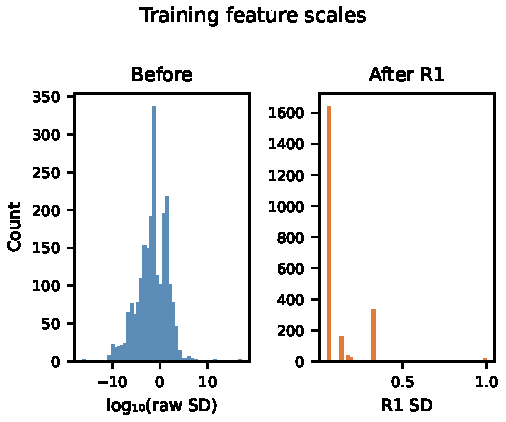
\includegraphics[width=\linewidth]{analysis/fig_before_after_scale.pdf}\captionof{figure}{The same selected training features before and after R1 preprocessing. Raw scales vary greatly; family weighting intentionally leaves unequal per-column standard deviations.}\end{center}

\section{Basic questions and problem statements}
Basic questions ask which subgenres have higher tempos, how brightness varies with tempo, and how often the extractor estimates minor mode. Our questions go beyond average profiles: they target within-subgenre multivariate spread, differences in feature relationships, and dependence-aware mode probabilities.

\textbf{P1 (primary).} Do subgenres differ in acoustic descriptor dispersion around their own centroids after training-fitted preprocessing? This concerns spread, not centroid location or artistic creativity.

\textbf{P2.} Does the association between tempo and spectral brightness have different slopes across subgenres after adjusting for extractor version?

\textbf{P3 (exploratory).} Do equal-cluster-weighted estimated minor-mode probabilities differ across subgenres?

\begin{center}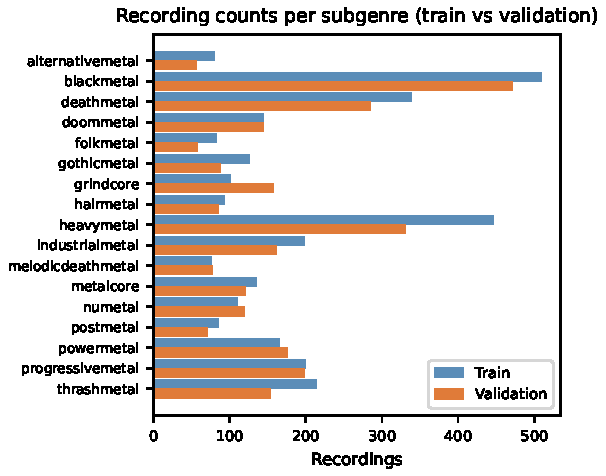
\includegraphics[width=\linewidth]{analysis/fig_subgenre_counts.pdf}\captionof{figure}{Recording counts are uneven across subgenres and splits; inference gives equal weight to dependence components within each subgenre.}\end{center}
\begin{center}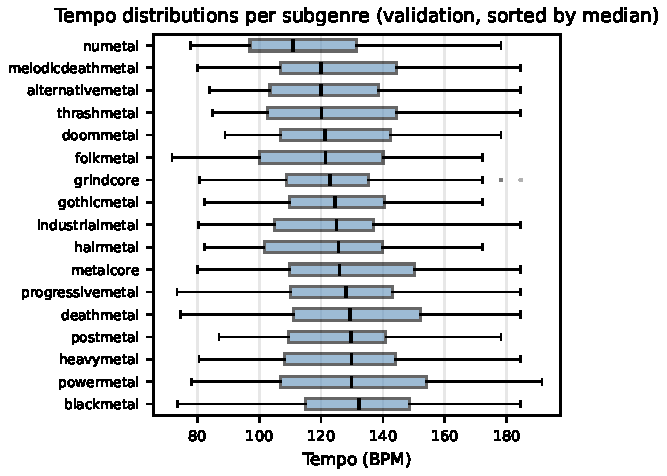
\includegraphics[width=\linewidth]{analysis/fig_tempo_by_subgenre.pdf}\captionof{figure}{Tempo distributions overlap and show substantial within-subgenre variation; a single group average does not describe every recording.}\end{center}
\begin{center}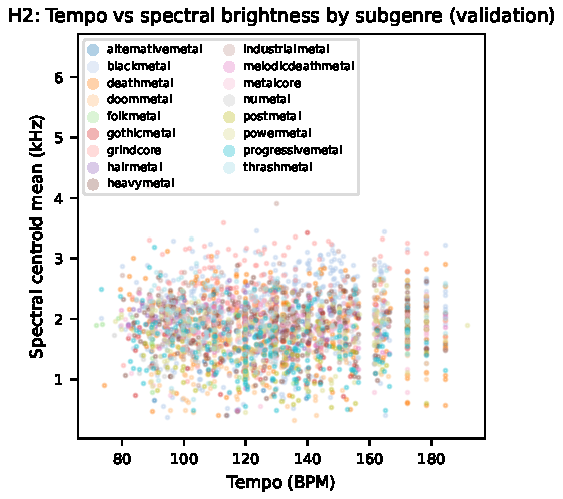
\includegraphics[width=\linewidth]{analysis/fig_bpm_sc_scatter.pdf}\captionof{figure}{Tempo and spectral brightness have broad, overlapping distributions. The slope test uses log scales and clustered uncertainty rather than reading a relationship from the raw scatter alone.}\end{center}

\section{Statistical inferences}
\minihead{Population, weighting and uncertainty}
All tests use the 2,754 validation recordings. For cluster $c$ in subgenre $g$, each observation has weight $w_i=1/(n_{cg}m_g)$, where $n_{cg}$ is its cluster--subgenre cell size and $m_g$ counts represented clusters. Weights sum to one within each subgenre. Validation subgenres have at least 25 components. Components crossing subgenres remain a single dependence unit.
H1 is primary at $\alpha=.05$. H2 and exploratory H3 form the two-test Holm family; sorted adjusted values use a cumulative maximum. All alternatives are omnibus (at least one difference); upper-tail Wald statistics do not imply a directional alternative. Intervals are 95\% and pointwise, not simultaneous post-hoc intervals.
The 10\% dispersion, 0.05 slope and 10-percentage-point mode benchmarks are \emph{project-defined SESOIs}, not established audible or psychoacoustic thresholds. They distinguish practical interpretation from a small $p$-value.

\subsection*{H1: multivariate acoustic dispersion}
\tpart{a}{Hypotheses and method}
$H_0:D_1=\cdots=D_{17}$; $H_A$: at least one differs. Here $D_g$ is the weighted mean Euclidean distance to the subgenre's own weighted centroid in R1.
We draw 1,999 whole-component bootstrap samples (seed 20261027), preserving every selected component's observations across subgenres. Repeated selections are separate occurrences; weights, centroids and distances are recomputed. The covariance $\widehat\Sigma$ of bootstrap $\log D$ gives
\[W=(A\log D)^\top(A\widehat\Sigma A^\top)^{-1}(A\log D),\]
where $A$ contains 16 independent equality contrasts. The reference is approximate $\chi^2_{16}$, \emph{not} an empirical permutation distribution. Percentile bootstrap intervals describe dispersions and the selected max/min ratio. Relative dispersion is $r_g=D_g/\exp[\operatorname{mean}(\log D)]$.

\tpart{b}{Why this method and alternatives}
Whole-component sampling preserves shared-artist dependence, including artists in several subgenres. PERMANOVA tests location, not our dispersion estimand; independent-track resampling ignores repeated recordings. Raw-label permutation can mix centroid differences into a dispersion comparison. The chosen bootstrap estimates uncertainty in the dispersion vector directly, with asymptotic Wald calibration.

\tpart{c}{Results and practical interpretation}
\begin{tabularx}{\linewidth}{@{}Y l@{}}\toprule
Statistic / quantity & Result\\\midrule
Wald $W$ (df) & 251.935 (16)\\
Approximate $p$ & $2.07\times10^{-44}$\\
Decision at .05 & Reject $H_0$\\
Max/min ratio & 1.359\\
Ratio 95\% interval & [1.311, 1.468]\\
Observed $r_g$ outside $[.90,1.10]$ & 4 of 17\\\bottomrule
\end{tabularx}
Black metal has the largest estimated dispersion, 8.600 (95\% CI 8.336--8.812); hair metal has the smallest, 6.328 (5.984--6.615). The ratio is substantial descriptively. Four relative point estimates exceed the chosen 10\% benchmark; these are not four adjusted significant contrasts. The selected ratio interval is descriptive and is not a simultaneous comparison of named pairs. Larger spread indicates more variable measured descriptors, not greater creativity.
The contrast covariance has rank 16 and condition number 44.95. All 1,999 bootstrap draws were usable; the Wald calibration remains asymptotic.
\begin{center}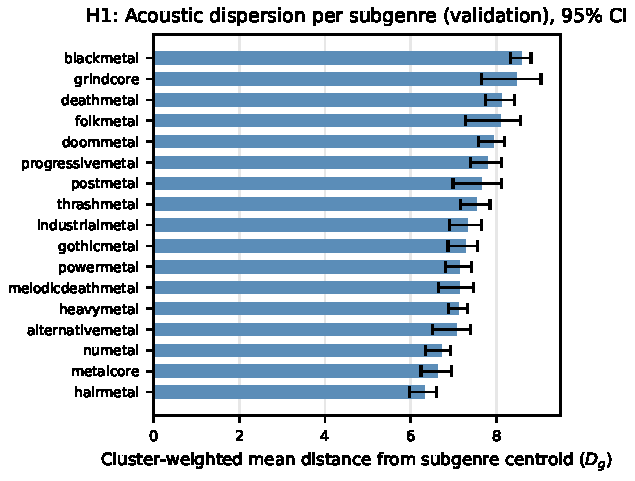
\includegraphics[width=\linewidth]{analysis/fig_dispersion_by_subgenre.pdf}\captionof{figure}{H1 dispersions with whole-component percentile intervals. Each distance is measured from its own subgenre centroid, separating spread from centroid location.}\end{center}

\subsection*{H2: tempo--brightness slope heterogeneity}
\tpart{a}{Hypotheses and method}
$H_0:\beta_1=\cdots=\beta_{17}$; $H_A$: at least one differs. Fit weighted least squares:
\[\log(\mathrm{centroid}_i)=\alpha_g+\beta_g x_i+\gamma I_{\mathrm{beta1},i}+\epsilon_i,\]
where $x_i=\log_2(\mathrm{BPM}_i/127.758)$ uses the training median. The covariance aggregates scores over whole components, with conventional CR1 correction $M/(M-1)\times(N-1)/(N-K)$. Here $M=1{,}004$, $N=2{,}754$, $K=35$. The slope-equality Wald reference is approximate $\chi^2_{16}$.
The pooled summary is the \emph{equal-subgenre average} $\bar\beta=c^\top\hat\beta$, $c_g=1/17$, not an imposed common slope. Its interval is $\bar\beta\pm1.96\sqrt{c^\top\widehat V_\beta c}$, preserving covariance between subgenre slopes.

\tpart{b}{Why this method and alternatives}
WLS matches the equal-component estimand; cluster scores allow correlated recordings and mixed-subgenre components. IID regression would ignore that dependence. A random-effects model requires an additional covariance/distribution specification; Spearman correlations concern monotonic association rather than the specified log-scale slope. CR1 is transparent but asymptotic and does not repair nonlinear specification or confounding.

\tpart{c}{Results and practical interpretation}
\begin{tabularx}{\linewidth}{@{}Y l@{}}\toprule
Statistic / quantity & Result\\\midrule
Wald $W$ (df) & 20.869 (16)\\
Raw / Holm $p$ & 0.1836 / 0.1836\\
Decision & Fail to reject $H_0$\\
Equal-subgenre average slope & +0.0164\\
95\% normal interval & [-0.0335, +0.0663]\\
Observed departures $>0.05$ & 10 of 17\\\bottomrule
\end{tabularx}
The average slope is small and its interval includes zero. A tempo doubling corresponds to an estimated 1.65\% brightness change on this equal-subgenre log-scale summary, with an interval of -3.30\% to 6.85\%. We do not establish equal slopes or a positive relationship. Ten slope point estimates differ from their average by more than .05, but this is a descriptive benchmark, not ten significant contrasts. The design has full rank 35; the contrast covariance has rank 16 and condition number 71.81.
\begin{center}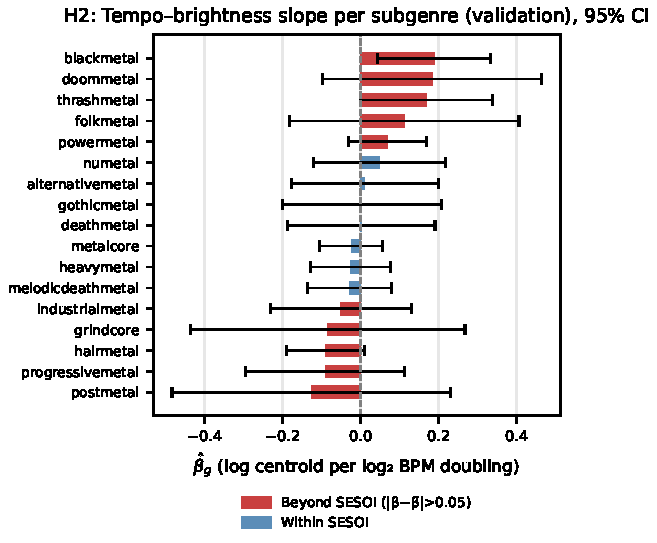
\includegraphics[width=\linewidth]{analysis/fig_slopes_by_subgenre.pdf}\captionof{figure}{Subgenre slopes with pointwise CR1 intervals. Red marks observed departures from the equal-subgenre average exceeding .05, not individually significant contrasts.}\end{center}

\subsection*{H3: estimated minor-mode association (exploratory)}
\tpart{a}{Hypotheses and method}
$H_0:p_1=\cdots=p_{17}$; $H_A$: at least one differs. A saturated weighted linear probability model has 17 subgenre indicators and no intercept. Its coefficients equal the weighted minor shares exactly. Whole-component CR1 covariance gives a 16-contrast Wald test with approximate $\chi^2_{16}$ reference. The 95\% intervals use the normal approximation; all lie within $[0,1]$.
This is a \emph{marginal} association, without extractor-version adjustment. H3 remains exploratory because validation mode counts were inspected during design.

\tpart{b}{Why this method and alternatives}
The saturated model directly estimates group probabilities, without requiring normally distributed binary responses. Track-level Pearson tests ignore dependence. Permuting whole labels is not justified when components contain several subgenres. Logistic regression is useful for conditional odds ratios, but is unnecessary for these marginal probability differences. The robust covariance still needs sufficiently many independent components.

\tpart{c}{Results and practical interpretation}
\begin{tabularx}{\linewidth}{@{}Y l@{}}\toprule
Statistic / quantity & Result\\\midrule
Wald $W$ (df) & 30.013 (16)\\
Raw / Holm $p$ & 0.0179 / 0.0359\\
Decision & Reject $H_0$ (exploratory)\\
Equal-subgenre mean share & 0.649\\
Observed share range & 0.418--0.805\\
Departures $>10$ percentage points & 3 of 17\\\bottomrule
\end{tabularx}
Hair metal has estimated minor share 0.418 (95\% CI 0.288--0.548); folk metal has 0.805 (0.686--0.925). The selected range is 38.75 percentage points, a descriptive extreme comparison. Three shares depart from the equal-subgenre mean by more than 10 points. This supports an exploratory association between tags and \emph{estimated} mode, not true musical key or compositional rules. Two mode estimators agree on only 60.8\% of retained recordings. The contrast covariance has rank 16 and condition number 45.04.
\begin{center}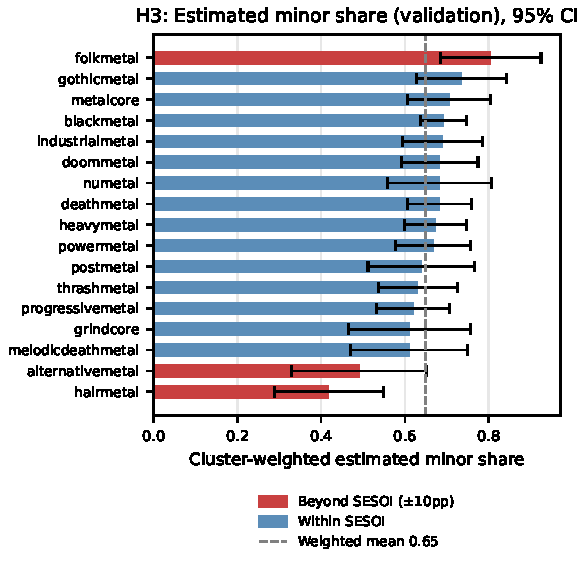
\includegraphics[width=\linewidth]{analysis/fig_minor_share.pdf}\captionof{figure}{Weighted minor shares with pointwise CR1 intervals. The dashed line is the same equal-subgenre weighted mean used in the results; red marks descriptive departures greater than 10 percentage points.}\end{center}

\section{Limitations and reproducibility}
\begin{itemize}
\item \textbf{Sampling and scope.} These are commercial recordings from selected downloaded shards, not a random sample of all metal. Crowd tags and extractor measurements are imperfect; associations are not causal.
\item \textbf{Dependence.} Connected components preserve observed shared-artist/album links. Missing or inaccurate identifiers can leave dependence between components. Some subgenres have only 25 components, so asymptotic Wald calibration warrants caution even with 1,004 total validation components.
\item \textbf{Split overlap.} The 348 shared components mean validation is not artist-independent of training. Uncertainty is conditional on training-fitted transformations, not a full two-stage sampling analysis. The original split was preserved.
\item \textbf{Representation.} Ranks compress tails; version correction removes location shifts only. Family definitions overlap acoustically. R2/R4 matrices are saved, but robustness across them was not tested.
\item \textbf{Inference.} Pointwise intervals do not justify simultaneous pairwise conclusions. Selected extrema and SESOI counts are descriptive. Numerical covariance screens are not a proof of statistical calibration; the very small H1 tail probability is an asymptotic approximation.
\item \textbf{Analysis history.} Implementation corrections were made after preliminary results had been inspected and are documented in the dated analysis-plan amendment. H3 is explicitly exploratory.
\end{itemize}
\field{Reproduction:}{The repository README describes the required extracted data, Python dependencies and execution order. The analysis scripts write numerical results, diagnostics and input hashes. Large raw and generated data arrays are not included in the repository; rerunning the analysis requires the extracted inputs described in the README.}
\field{Code availability:}{Code, numerical summaries, figures and report sources are available in the \href{https://github.com/Swarnav-Chakma/Metal-music-statistical-analysis}{public GitHub repository}. The report source is \path{CSE558_Midterm_Report.tex}; \path{report.tex} and both PDFs are synchronized copies.}
\end{document}